\documentclass[conference]{IEEEtran}
\IEEEoverridecommandlockouts
\usepackage{cite}
\usepackage{amsmath,amssymb,amsfonts}
\usepackage{algorithmic}
\usepackage{graphicx}
\usepackage{textcomp}
\usepackage{xcolor}
\usepackage{caption}
\usepackage{subcaption}

\def\BibTeX{{\rm B\kern-.05em{\sc i\kern-.025em b}\kern-.08em
T\kern-.1667em\lower.7ex\hbox{E}\kern-.125emX}}

\graphicspath{{../results_20240625-175613/}{../}}
% Setting global graphics path

\begin{document}

\begin{figure}[htbp]
    \centering
    \begin{subfigure}{.2\textwidth}
        \centering
        \includegraphics[width=\linewidth]{input_image.png}
        \subcaption{Image}
    \end{subfigure}
    \hfill
    \begin{subfigure}{.2\textwidth}
        \centering
        \includegraphics[width=\linewidth]{input_label.png}
        \subcaption{Label}
    \end{subfigure}
    \caption{Example Images and Labels}
    \label{fig:images}
\end{figure}

\begin{figure}[htbp]
    \centering
    \begin{subfigure}{.2\textwidth}
        \centering
        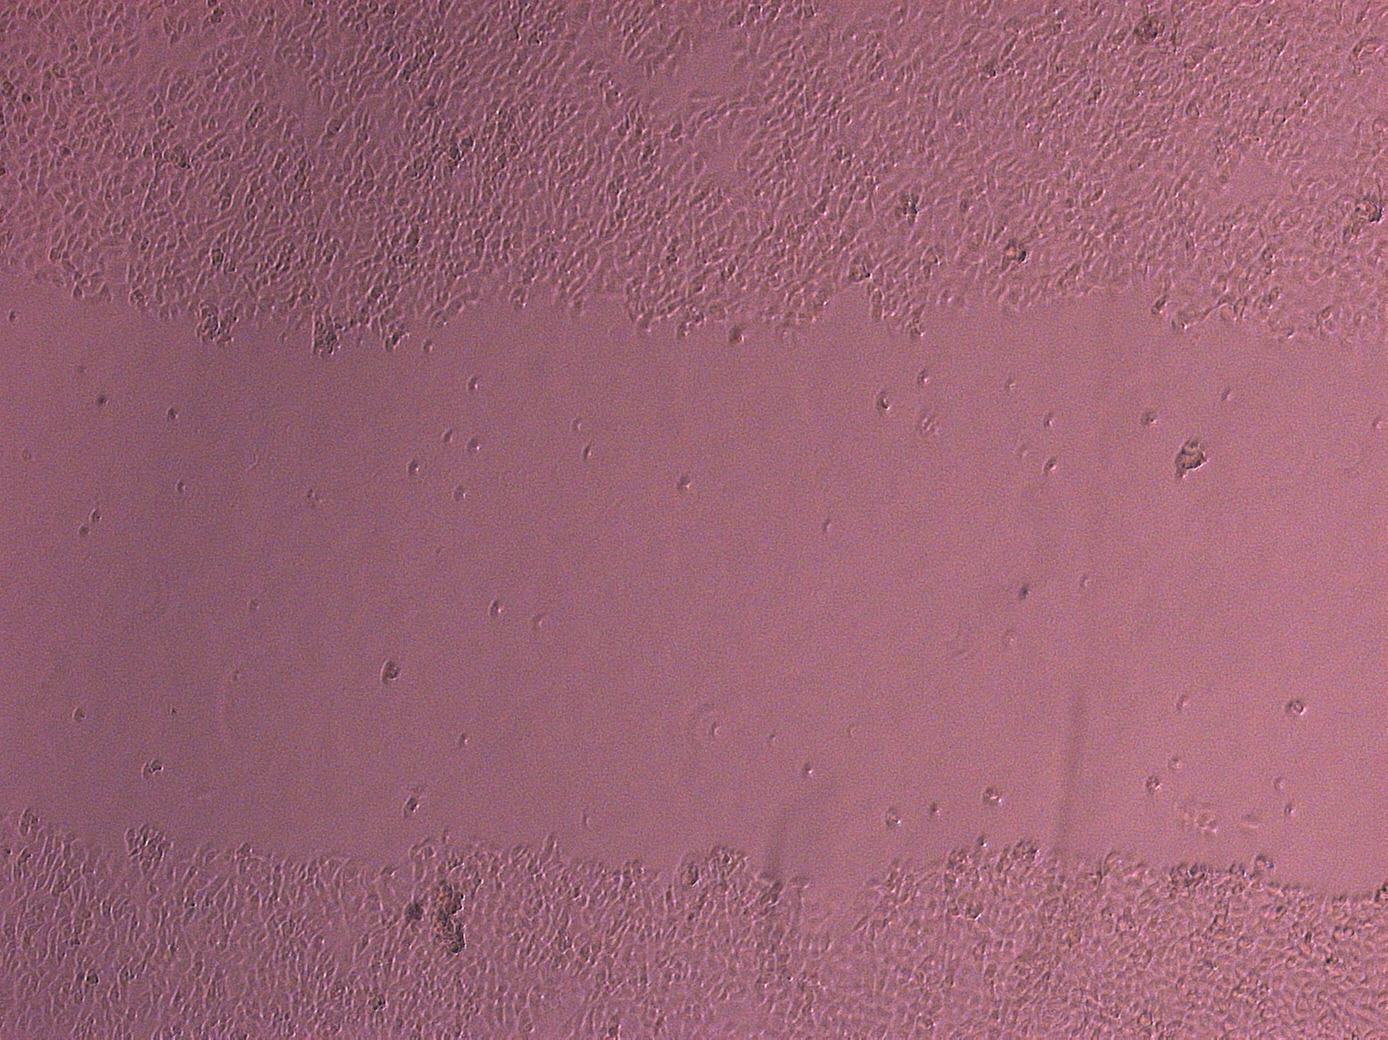
\includegraphics[width=\linewidth]{0h.png}
        \subcaption{0h}
    \end{subfigure}
    \hfill
    \begin{subfigure}{.2\textwidth}
        \centering
        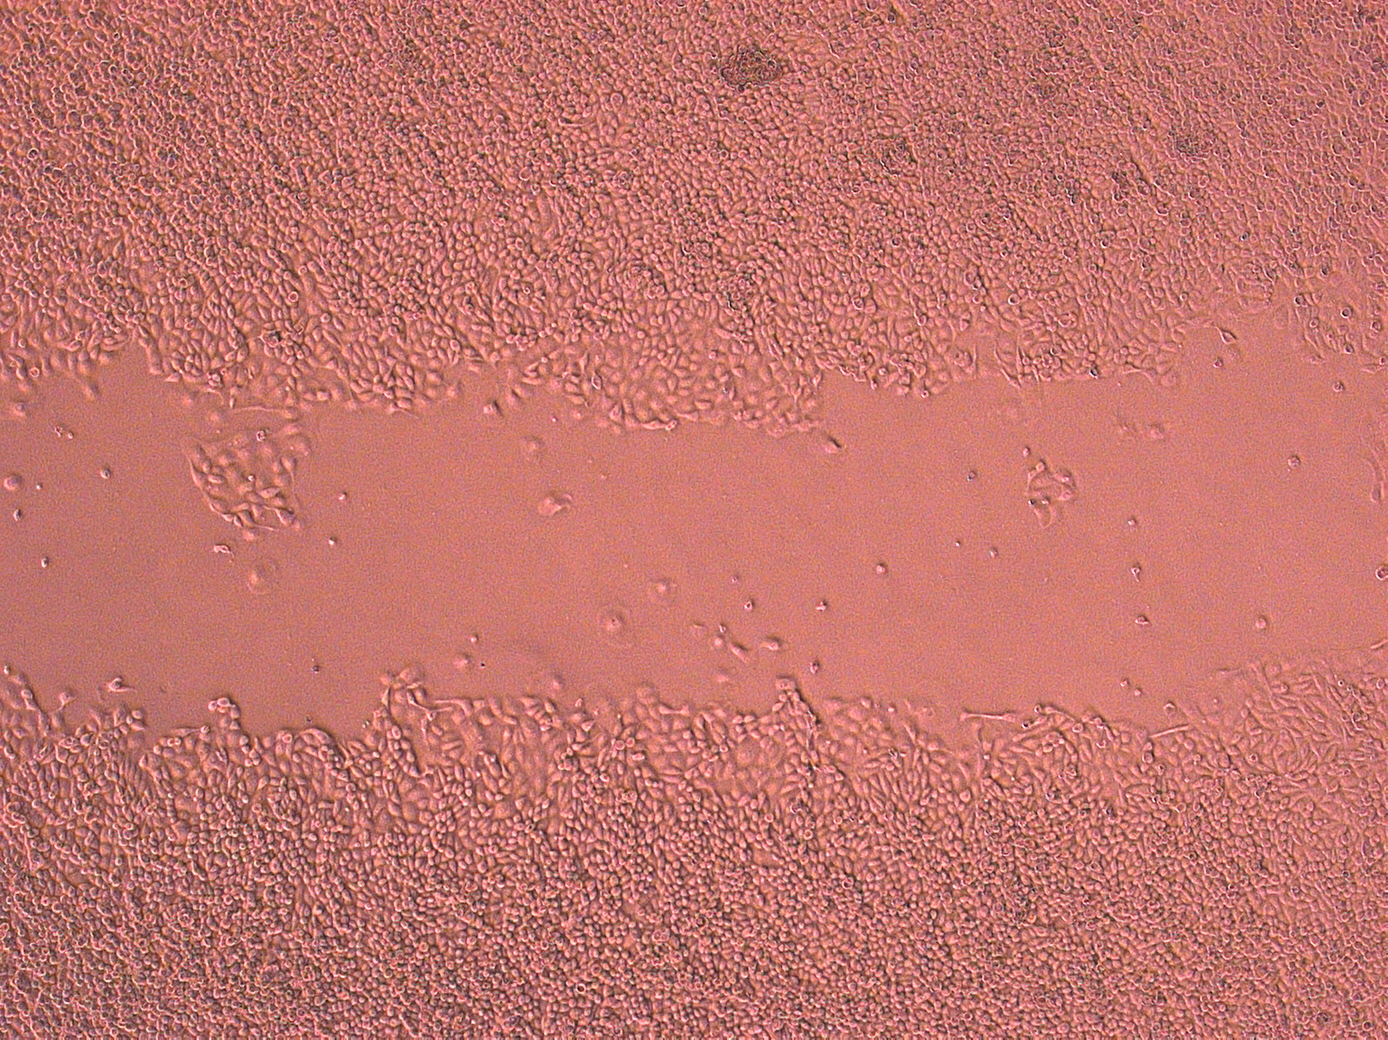
\includegraphics[width=\linewidth]{24h.png}
        \subcaption{24h}
    \end{subfigure}
    \hfill
    \begin{subfigure}{.2\textwidth}
        \centering
        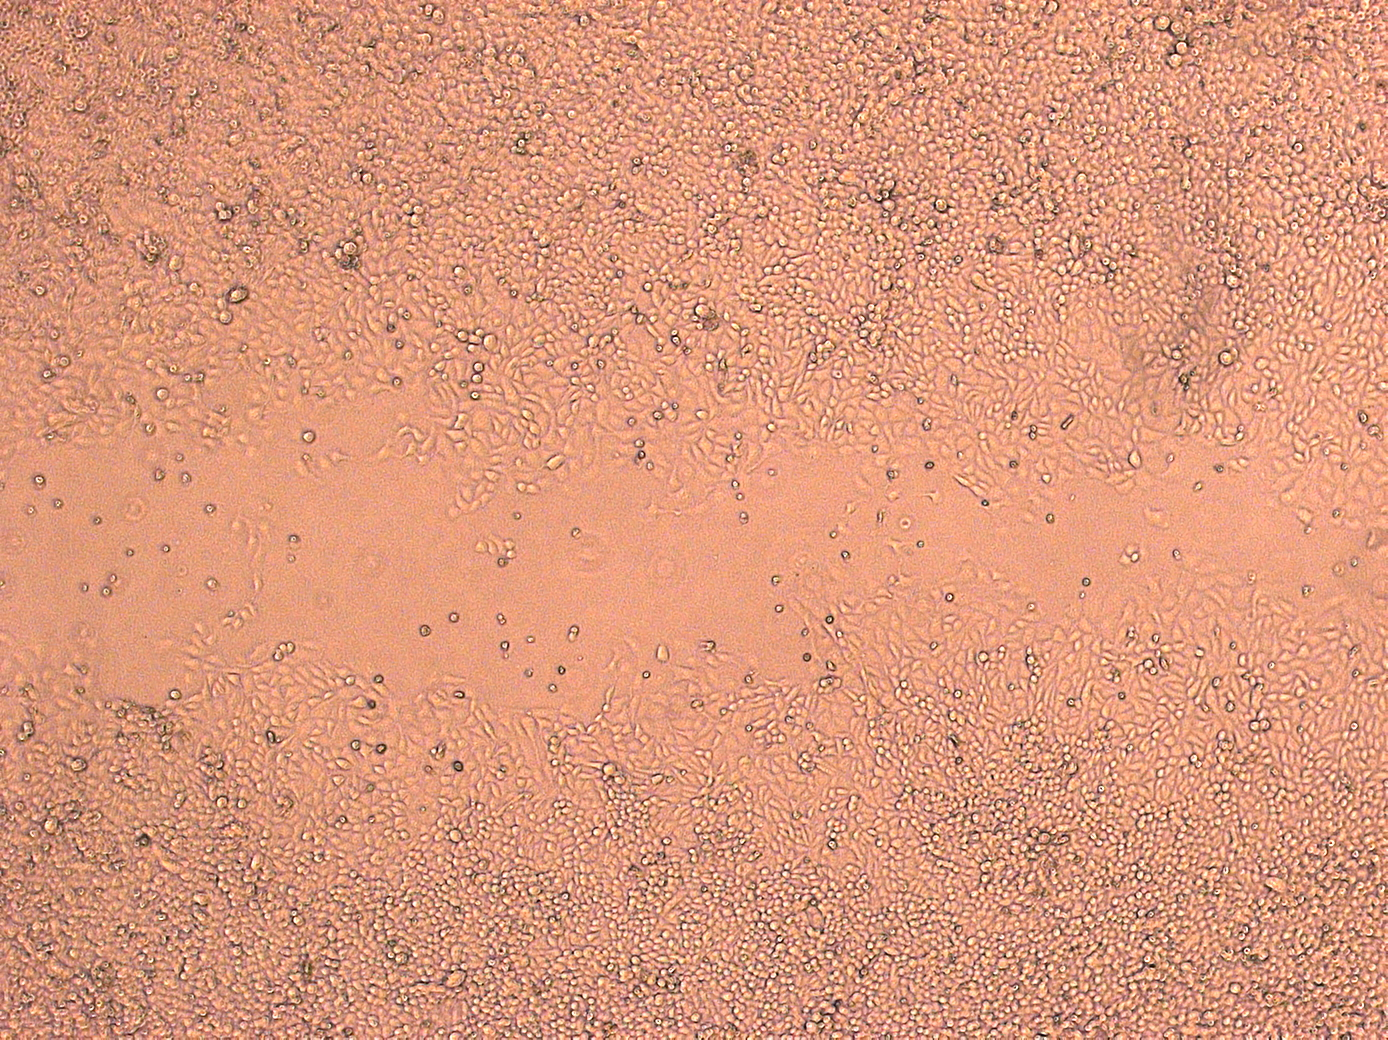
\includegraphics[width=\linewidth]{48h.png}
        \subcaption{48h}
    \end{subfigure}
    \hfill
    \begin{subfigure}{.2\textwidth}
        \centering
        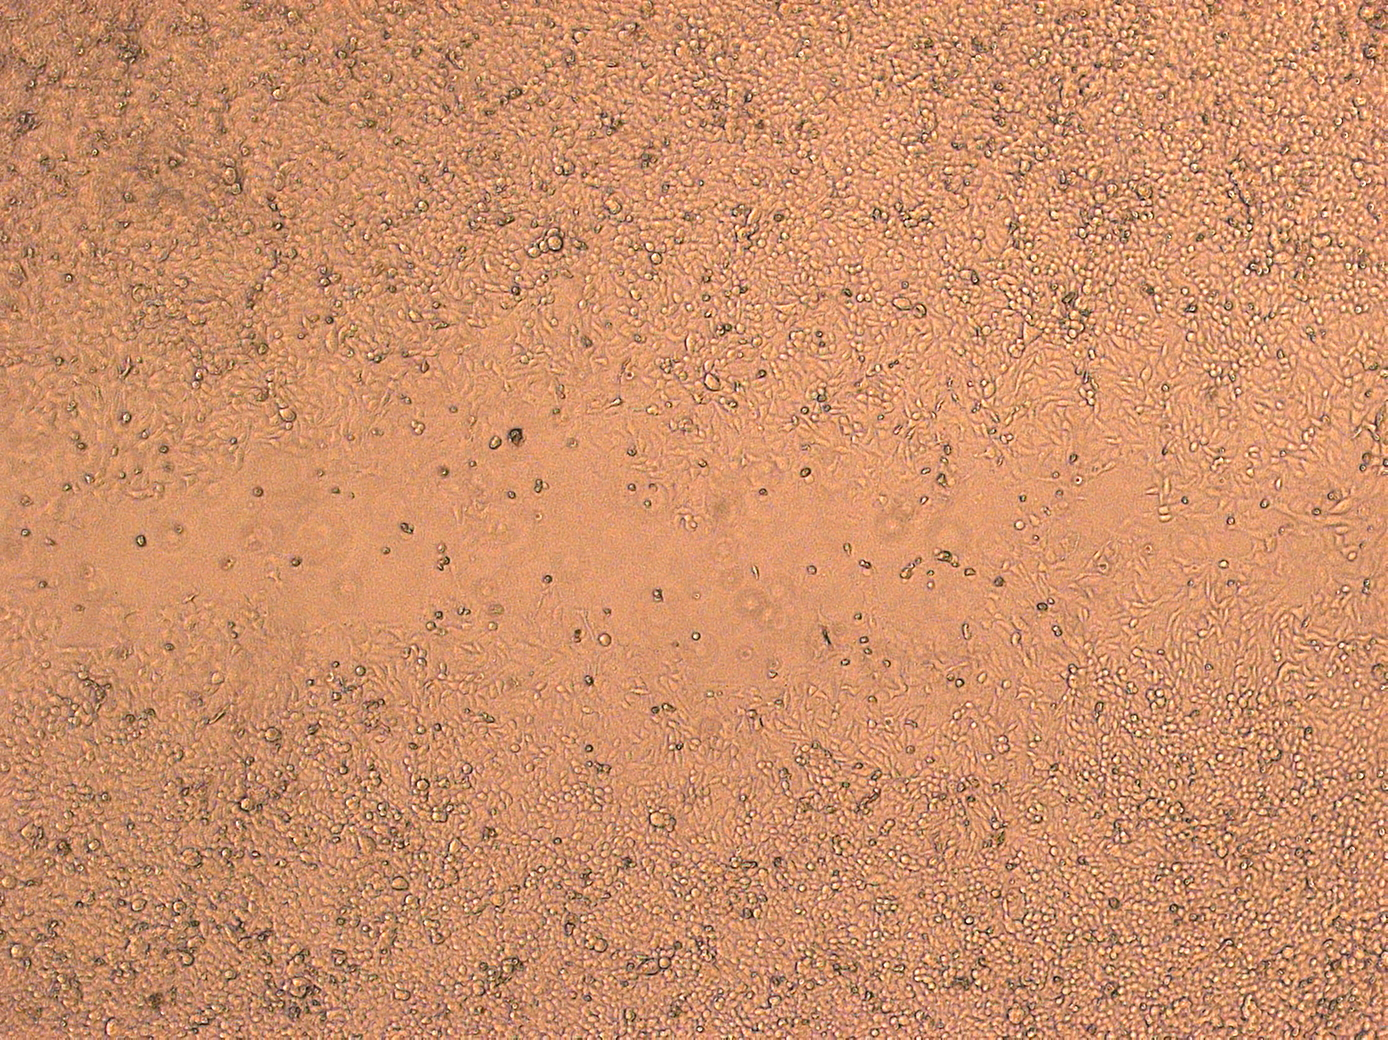
\includegraphics[width=\linewidth]{72h.png}
        \subcaption{72h}
    \end{subfigure}
    \caption{Time Series Images}
    \label{fig:images2}
\end{figure}

\begin{table}[htbp]
    \centering
    \caption{HuTu-80 Dataset Characteristics}
    \begin{tabular}{c|c}
        \hline
        \textbf{\# of Samples}  & 180 Images   \\
        \hline
        \textbf{Size of Image}  & (1048, 1388) \\
        \hline
        \textbf{\# of Channels} & 3 (RGB)      \\
        \hline
    \end{tabular}
    \label{tab:dataset_details}
\end{table}

\end{document}
